\begin{dang}{Tìm các đường tiệm cận đồ thị hàm ẩn}
\end{dang}
\begin{vd}
    Cho hàm số $y=f(x)$ có bảng biến thiên như hình vẽ sau
    \begin{center}
        
\begin{tikzpicture}[>=stealth]
            \tkzTabInit[nocadre=false,lgt=1,espcl=1.5,deltacl=0.5]{$x$/.7 ,$y'$/.7,$y$/2}
            {$-\infty$ , $-1$ , $2$ , $+\infty$}
            \tkzTabLine{ , + , $0$ , - , d , + , }
            \tkzTabVar{-/$1$ , +/$4$ , -/$-5$ , +/$+\infty$}
        \end{tikzpicture}
    \end{center}
    Tìm TCĐ, TCN của đồ thị hàm số
    \begin{listEX}[3]
        \item $y=\dfrac{2}{f(x)-3}$
        \item $y=\dfrac{-3}{f(x)+2}$
        \item $y=\dfrac{x-2}{f(x)+5}$
        \item $y=\dfrac{x+1}{f(x)-4}$
        \item $y=\dfrac{2}{f(x^2)+3}$
        \item $y=\dfrac{4f(x)-5}{3f(x)+1}$
    \end{listEX}
    \loigiai{}
\end{vd}
\begin{vd}\immini{Cho hàm bậc ba $y=f(x)$ có đồ thị như hình vẽ. Tìm số tiệm cận đứng của đồ thị hàm số
        \begin{listEX}[2]
            \item $y=\dfrac{\sqrt{x+3}}{(x-1)f(x)}$
            \item $g(x)=\dfrac{(x^2+4x+3)\sqrt{x^2+x}}{x\left[f^2(x)-2f(x)\right]}$ .
    \end{listEX}}{\begin{tikzpicture}[line cap=round,line join=round, >=stealth,font=\footnotesize]
            \begin{scope}[scale=.5]
                \def\a{-1} % Hệ số a phải khác 0
                \def\b{-13/2}
                \def\c{-12}
                \def\d{-9/2}
                \draw[->] (-5,0) -- (2,0)node[below]{$x$};
                \draw[->] (0,-3) -- (0,4) node[left] {$y$};
                \draw (0,0)node[below right]{$O$} (-3,0)node[below]{$-3$};
                \draw[dashed] (-1,0)node[below]{$-1$}|-(0,2)node[right]{$2$};
                \draw[samples=150,smooth,domain=-4:.-.2] plot(\x,{\a*(\x)^3+(\b)*(\x)^2+(\c)*\x+(\d)});
            \end{scope}
    \end{tikzpicture}}
    \loigiai{
        \begin{center}
            \begin{tikzpicture}[line cap=round,line join=round, >=stealth,font=\footnotesize,scale=1]
                \def\a{-1} % Hệ số a phải khác 0
                \def\b{-13/2}
                \def\c{-12}
                \def\d{-9/2}
                \draw[->] (-5,0) -- (2,0)node[below]{$x$};
                \draw[->] (0,-3) -- (0,4) node[left] {$y$};
                \draw (0,0)node[below right]{$O$} (-3,0)node[below]{$-3$} (-.3,0)node[above]{$a$};
                \draw[dashed] (-3.78,0)node[below]{$c$}|-(0,2)|-(-1.71,0)node[below]{$b$}|-(0,2) (-1,0)node[below]{$-1$}|-(0,2)node[right]{$2$};
                \draw[samples=150,smooth,domain=-4:.-.2] plot(\x,{\a*(\x)^3+(\b)*(\x)^2+(\c)*\x+(\d)});
            \end{tikzpicture}
        \end{center}
        $g(x)=\dfrac{(x^2+4x+3)\sqrt{x^2+x}}{x\left[f^2(x)-2f(x)\right]}=\dfrac{(x+1)(x+3)\sqrt{x(x+1)}}{x\left[f^2(x)-2f(x)\right]}$.\\
        Điều kiện của căn là $x\le -1; x\ge 0$.\\
        Dựa vào đồ thị ta có \[x\left[f^2(x)-2f(x)\right]=0 \Leftrightarrow \hoac{&x=0\\&f(x)=0\\& f(x)=2} \Leftrightarrow \hoac{&x=0\text{ (nhận)}\\&x=-3\text{ (nhận)};\ x=a \text{ (loại)} \\&x=-1\text{ (nhận)};\ x=b\text{ (nhận)};\ x=c\text{ (nhận)}}\]\\
        Số TCĐ lúc này chính là số nghiệm không bị rút gọn của mẫu, vậy có bốn TCĐ là $x=0; x=-3; x=b; x=c$.
    }
\end{vd}
\BTTN
\Opensolutionfile{ans}[ans/2D1-4-DANG-3]
\begin{ex}%[2D1K4-1]
    Cho hàm số $y=f(x)$ có bảng biến thiên như hình bên. Đồ thị hàm số $y=\dfrac{-5}{f(x)+4}$ có bao nhiêu tiệm cận đứng?
    \begin{center}
        
\begin{tikzpicture}[scale=0.8]
            \tkzTabInit[nocadre=false,lgt=1.5,espcl=3,deltacl=0.6]
            {$x$ /0.6,$y’$ /0.6,$y$ /2}
            {$-\infty$ ,$1$, $2$, $+\infty$}
            \tkzTabLine{,+,d,-,d,+,}
            \tkzTabVar{-/$-4$,+/$3$,-/$-5$,+/$+\infty$}
        \end{tikzpicture}
    \end{center}
    \choice
    {$1$}
    {$3$}
    {\True $2$}
    {$4$}
    \loigiai{
        Dựa vào bảng biến thiên suy ra
        $f(x)+4=0 \Leftrightarrow f(x) =-4$, phương trình này có $2$ nghiệm phân biệt nên đồ thị hàm số $y=\dfrac{-5}{f(x)+4}$ có $2$ tiệm cận đứng.
    }
\end{ex}
\begin{ex}%[2D1K4-1]
    Cho hàm số $y=f(x)$ có bảng biến thiên như hình bên. Đồ thị hàm số $y=\dfrac{x+2}{2f(x)-1}$ có bao nhiêu tiệm cận đứng?
    \begin{center}
        
\begin{tikzpicture}[scale=0.8]
            \tkzTabInit[nocadre=false,lgt=1.5,espcl=3,deltacl=0.6]
            {$x$ /0.6,$y’$ /0.6,$y$ /2}
            {$-\infty$ ,$-1$, $0$, $1$, $+\infty$}
            \tkzTabLine{,+,0,-,0,+,0,-,}
            \tkzTabVar{-/$-\infty$,+/$0$,-/$-\dfrac{5}{3}$,+/$0$,-/$-\infty$}
        \end{tikzpicture}
    \end{center}
    \choice
    {$1$}
    {$3$}
    {$2$}
    {\True $0$}
    \loigiai{
        Dựa vào bảng biến thiên suy ra
        $2f(x)-1=0 \Leftrightarrow f(x) =\dfrac{1}{2}$, phương trình này có $0$ nghiệm nên đồ thị hàm số $y=\dfrac{x+2}{2f(x)-1}$ không có tiệm cận đứng.
    }
\end{ex}
%69
\begin{ex}%[2D1K4-1]
    Cho hàm số $y=f(x)$ có bảng biến thiên như hình bên. Đồ thị hàm số $y=\dfrac{1}{2f(x)-3}$ có bao nhiêu tiệm cận đứng?
    \begin{center}
        
\begin{tikzpicture}[scale=0.8]
            \tkzTabInit[nocadre=false,lgt=1.5,espcl=3,deltacl=0.6]
            {$x$ /0.6,$y’$ /0.6,$y$ /2}
            {$-\infty$ ,$0$, $1$, $+\infty$}
            \tkzTabLine{,+,0,-,0,+,}
            \tkzTabVar{-/$-\infty$,+/$5$,-/$-1$,+/$+\infty$}
        \end{tikzpicture}
    \end{center}
    \choice
    {$1$}
    {\True $3$}
    {$2$}
    {$0$}
    \loigiai{
        Dựa vào bảng biến thiên suy ra
        $2f(x)-3=0 \Leftrightarrow f(x) =-\dfrac{3}{2}$, phương trình này có $3$ nghiệm phân biệt nên đồ thị hàm số $y=\dfrac{1}{2f(x)-3}$ có ba tiệm cận đứng.
    }
\end{ex}
%70
%71
%72
\begin{ex}%[2D1K4-1]
    Cho hàm số $y=f(x)$ có bảng biến thiên như hình bên. Đồ thị hàm số $y=\dfrac{x}{f(x)-3}$ có bao nhiêu tiệm cận đứng?
    \begin{center}
        
\begin{tikzpicture}[scale=0.8]
            \tkzTabInit[nocadre=false,lgt=1.5,espcl=3,deltacl=0.6]
            {$x$ /0.6,$y’$ /0.6,$y$ /2}
            {$-\infty$ ,$-1$, $0$, $1$, $+\infty$}
            \tkzTabLine{,-,0,+,0,-,0,+,}
            \tkzTabVar{+/$+\infty$,-/$0$,+/$3$,-/$0$,+/$+\infty$}
        \end{tikzpicture}
    \end{center}
    \choice
    {$1$}
    {\True $3$}
    {$2$}
    {$4$}
    \loigiai{
        Dựa vào bảng biến thiên suy ra
        $f(x)-3=0 \Leftrightarrow f(x) =3$, phương trình này có $2$ nghiệm phân biệt khác $0$ và một nghiệm bội chẵn $x=0$ nên đồ thị hàm số $y=\dfrac{x}{f(x)-3}$ có ba tiệm cận đứng.
    }
\end{ex}
\begin{ex}%[2D1K4-1]
    Cho hàm số $y=f(x)$ có bảng biến thiên như hình bên. Đồ thị hàm số $y=\dfrac{4}{f(x)+1}$ có tiệm cận ngang là đường thẳng
    \begin{center}
        
\begin{tikzpicture}[scale=0.8]
            \tkzTabInit[nocadre=false,lgt=1.5,espcl=3,deltacl=0.6]
            {$x$ /0.6,$y’$ /0.6,$y$ /2}
            {$-\infty$ ,$-1$, $2$, $+\infty$}
            \tkzTabLine{,+,0,-,0,+,}
            \tkzTabVar{-/$1$,+/$4$,-/$-5$,+/$1$}
        \end{tikzpicture}
    \end{center}
    \choice
    {$y=1$}
    {$y=-5$}
    {\True $y=2$}
    {$y=4$}
    \loigiai{
        Dựa vào bảng biến thiên suy ra
        $\lim \limits_{x \to \pm \infty} f(x)=1 \Leftrightarrow \lim \limits_{x \to \pm \infty} \dfrac{4}{f(x)+1} =2$ nên đồ thị hàm số đã cho có tiệm cận ngang là $y=2$.
    }
\end{ex}
\begin{ex}%[2D1K4-1]
    Cho hàm số $y=f(x)$ có bảng biến thiên như hình bên. Đồ thị hàm số $y=\dfrac{2-f(x)}{f(x)+3}$ có tiệm cận ngang là đường thẳng
    \begin{center}
        
\begin{tikzpicture}[scale=0.8]
            \tkzTabInit[nocadre=false,lgt=1.5,espcl=3,deltacl=0.6]
            {$x$ /0.6,$y’$ /0.6,$y$ /2}
            {$-\infty$ ,$0$, $2$, $+\infty$}
            \tkzTabLine{,-,0,+,0,-,}
            \tkzTabVar{+/$+\infty$,-/$1$,+/$5$,-/$-\infty$}
        \end{tikzpicture}
    \end{center}
    \choice
    {$y=1$}
    {$y=-3$}
    {$y=2$}
    {\True $y=-1$}
    \loigiai{
        Dựa vào bảng biến thiên suy ra
        $\lim \limits_{x \to \pm \infty} f(x)=\pm \infty \Leftrightarrow \lim \limits_{x \to \pm \infty} \dfrac{2-f(x)}{f(x)+3} =-1$ nên đồ thị hàm số $y=\dfrac{2-f(x)}{f(x)+3}$ có tiệm cận ngang là $y=-1$.
    }
\end{ex}
\begin{ex}%[2D1K4-1]
    Cho hàm số $y=f(x)$ có bảng biến thiên như hình bên. Đồ thị hàm số $y=\dfrac{1}{f^2(x)-4f(x)+4}$ có bao nhiêu tiệm cận đứng?
    \begin{center}
        
\begin{tikzpicture}[scale=0.8]
            \tkzTabInit[nocadre=false,lgt=1.5,espcl=3,deltacl=0.6]
            {$x$ /0.6,$y’$ /0.6,$y$ /2}
            {$-\infty$, $2$, $+\infty$}
            \tkzTabLine{,-,0,+,}
            \tkzTabVar{+/$1$,-/$-3$,+/$1$}
        \end{tikzpicture}
    \end{center}
    \choice
    {$1$}
    {$3$}
    {$2$}
    {$0$}
    \loigiai{
        Dựa vào bảng biến thiên suy ra $f^2(x)-4f(x)+4=0 \Leftrightarrow f(x)=2$, phương trình $f(x)=2$ vô nghiệm nên đồ thị hàm số đã cho không có tiệm cận đứng.
    }
\end{ex}
%83
\begin{ex}%[2D1K4-1]
    Cho hàm số $y=f(x)$ có bảng biến thiên như hình bên. Đồ thị hàm số $y=\dfrac{1}{f(3-x)-2}$ có bao nhiêu tiệm cận đứng?
    \begin{center}
        
\begin{tikzpicture}[scale=0.8]
            \tkzTabInit[nocadre=false,lgt=1.5,espcl=3,deltacl=0.6]
            {$x$ /0.6,$y’$ /0.6,$y$ /2}
            {$-\infty$ ,$-2$, $2$, $+\infty$}
            \tkzTabLine{,+,0,-,0,+,}
            \tkzTabVar{-/$-\infty$,+/$3$,-/$0$,+/$+\infty$}
        \end{tikzpicture}
    \end{center}
    \choice
    {$1$}
    {\True $3$}
    {$2$}
    {$0$}
    \loigiai{
        Dựa vào bảng biến thiên suy ra $f(3-x)-2=0 \Leftrightarrow f(3-x)=2$, phương trình này có $3$ nghiệm phân biệt nên đồ thị hàm số đã cho có $3$ tiệm cận đứng.
    }
\end{ex}
\begin{ex}%[2D1G4-1]
    Cho hàm số $y=f(x)$ có bảng biến thiên như hình bên. Đồ thị hàm số $y=\dfrac{4}{f(x^2)-2}$ có bao nhiêu tiệm cận đứng?
    \begin{center}
        
\begin{tikzpicture}[scale=0.8]
            \tkzTabInit[nocadre=false,lgt=1.5,espcl=3,deltacl=0.6]
            {$x$ /0.6,$y’$ /0.6,$y$ /2}
            {$-\infty$ ,$0$, $3$, $+\infty$}
            \tkzTabLine{,-,0,+,d,-,}
            \tkzTabVar{+/$8$,-/$1$,+/$4$,-/$2$}
        \end{tikzpicture}
    \end{center}
    \choice
    {$5$}
    {$3$}
    {\True $2$}
    {$4$}
    \loigiai{
        Dựa vào bảng biến thiên suy ra
        $f(x^2)-2=0 \Leftrightarrow f(x^2) =2$. Kẻ đường thẳng $y=2$ ta thấy đường thẳng cắt đồ thị hàm số tại hai điểm phân biệt. Suy ra
        $$\hoac{&x^2=a \; (a<0)\\&x^2=b \; (b >0)} \Rightarrow x=\pm \sqrt{b}.$$
        Do đó đồ thị hàm số đã cho có $2$ tiệm cận đứng.
    }
\end{ex}%89
\begin{ex}%[2D1G4-1]
    Cho hàm số $y=f(x)$ có bảng biến thiên như hình bên. Đồ thị hàm số $y=\dfrac{2}{f(|x|)-3}$ có bao nhiêu tiệm cận ngang?
    \begin{center}
        
\begin{tikzpicture}[scale=0.8]
            \tkzTabInit[nocadre=false,lgt=1.5,espcl=3,deltacl=0.6]
            {$x$ /0.6,$y’$ /0.6,$y$ /2}
            {$-\infty$ ,$0$, $2$, $+\infty$}
            \tkzTabLine{,+,0,-,0,+,}
            \tkzTabVar{-/$-\infty$,+/$3$,-/$-1$,+/$+\infty$}
        \end{tikzpicture}
    \end{center}
    \choice
    {$4$}
    {\True $3$}
    {$5$}
    {$6$}
    \loigiai{
        Dựa vào bảng biến thiên suy ra
        $f(|x|)-3=0 \Leftrightarrow f(|x|) =3$.\\
        Bảng biến thiên hàm số $y=f(|x|)$ như sau
        \begin{center}
            
\begin{tikzpicture}[scale=0.8]
                \tkzTabInit[nocadre=false,lgt=1.5,espcl=3,deltacl=0.6]
                {$x$ /0.6,$y’$ /0.6,$y$ /2}
                {$-\infty$ ,$-2$, $0$, $2$, $+\infty$}
                \tkzTabLine{,-,0,+,0,-,0,+,}
                \tkzTabVar{+/$+\infty$,-/$-1$,+/$3$,-/$-1$,+/$+\infty$}
            \end{tikzpicture}
        \end{center}
        Dựa vào bảng biến thiên hàm số $y=f(|x|)$, phương trình $f(|x|) =3$ có ba nghiệm phân biệt, do đó đồ thị hàm số $y=\dfrac{2}{f(|x|)-3}$ có $3$ tiệm cận đứng.
    }
\end{ex}
\begin{ex}
    \immini{ %Câu 90
        Cho hàm số bậc ba $f(x)= ax^3 +bx^2 +cx +d$ có đồ thị như hình vẽ bên. Đồ thị hàm số $g(x) = \dfrac{\sqrt{x+1}}{(x-3)\cdot f(x)}$ có bao nhiêu đường tiệm cận đứng?
        \choice
        {5}
        {2}
        {4}
        {\True 3}}{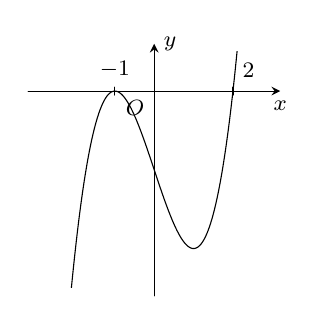
\begin{tikzpicture}[scale=.5, font=\footnotesize, line join=round, line cap=round, >=stealth]
            \def\xmin{-3}\def\xmax{3}\def\ymin{-5}\def\ymax{1}
            \draw[->] (\xmin-0.2,0)--(\xmax+0.2,0) node[below] {\footnotesize $x$};
            \draw[->] (0,\ymin-0.2)--(0,\ymax+0.2) node[right] {\footnotesize $y$};
            \draw (0,0) node [below left] {\footnotesize $O$};
            \foreach \x in {-1}\draw (\x,-0.1)--(\x,0.1) node [above] {\footnotesize $\x$};
            \foreach \x in {2}\draw (\x,-0.1)--(\x,0.1) node [above right] {\footnotesize $\x$};
            \foreach \y in {}\draw (-0.1,\y)--(0.1,\y) node [right] {\footnotesize $\y$};
            \clip (\xmin,\ymin) rectangle (\xmax,\ymax);
            \draw[smooth,samples=200,domain=\xmin:\xmax] plot (\x,{1*((\x)^3)+0*((\x)^2)+-3*(\x)+-2});
        \end{tikzpicture}
    }
    \loigiai{
        * Điều kiện: $\heva{&x \ne 3\\&f(x) \ne 0\\&x \ge -1.}$\\
        Nhìn hình vẽ ta thấy
        $f(x)=0\Leftrightarrow \hoac{&x=-1&(\text{nghiệm kép}) \\&x=2&(\text{nghiệm đơn}).}$\\
        Vậy $g(x) = \dfrac{\sqrt{x+1}}{(x-3)\cdot a(x+1)^2 (x-2)}.$ \\
        Đồ thị hàm số $g(x)$ có 3 đường tiệm cận đứng.}
\end{ex}
\begin{ex}
    \immini{ %Câu 92.
        Đường cong ở hình bên là đồ thị của hàm số $y = ax^3 +bx^2 +cx+d$. Đồ thị hàm số $y =\dfrac{(2x+1)\sqrt{x-1}}{x\cdot f(x-2)}$ có tất cả bao nhiêu tiệm cận đứng?
        \choice
        {1}
        {3}
        {4}
        {\True 2}}{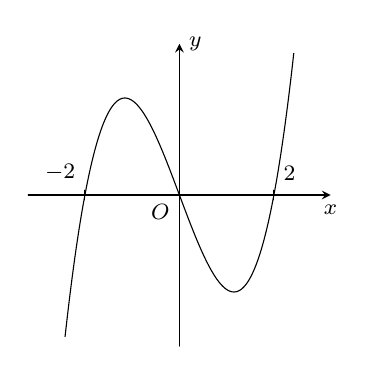
\begin{tikzpicture}[scale=.6, font=\footnotesize, line join=round, line cap=round, >=stealth]
            \def\xmin{-3}\def\xmax{3}\def\ymin{-3}\def\ymax{3}
            \draw[->] (\xmin-0.2,0)--(\xmax+0.2,0) node[below] {\footnotesize $x$};
            \draw[->] (0,\ymin-0.2)--(0,\ymax+0.2) node[right] {\footnotesize $y$};
            \draw (0,0) node [below left] {\footnotesize $O$};
            \foreach \x in {-2}\draw (\x,-0.1)--(\x,0.1) node [above left] {\footnotesize $\x$};
            \foreach \x in {2}\draw (\x,-0.1)--(\x,0.1) node [above right] {\footnotesize $\x$};
            \foreach \y in {}\draw (-0.1,\y)--(0.1,\y) node [right] {\footnotesize $\y$};
            \clip (\xmin,\ymin) rectangle (\xmax,\ymax);
            \draw[smooth,samples=200,domain=\xmin:\xmax] plot (\x,{(2/3)*((\x)^3)+0*((\x)^2)+-(8/3)*(\x)});
    \end{tikzpicture}}
    \loigiai{
        * Điều kiện: $\heva{&x \ne 0\\&f(x-2) \ne 0\\&x \ge 1.}$\\
        Nhìn hình vẽ ta thấy
        $f(x-2)=0\Leftrightarrow \hoac{&x-2=-2\\&x-2=0\\&x-2=2}\Leftrightarrow \hoac{&x=0&(\text{không thỏa mãn})\\&x=2&(\text{nghiệm đơn})\\&x=4&(\text{nghiệm đơn}).}$\\
        Vậy $g(x) =\dfrac{(2x+1)\sqrt{x-1}}{x\cdot f(x-2)}=\dfrac{(x-1)\sqrt{x+2}}{x\cdot ax(x-2)(x-4)}.$ \\
        Đồ thị hàm số $g(x)$ có 2 đường tiệm cận đứng.}
\end{ex}
\begin{ex}
    \immini{ %Câu 93.
        Cho hàm số $y= f(x)$ có đồ thị cắt trục hoành tại đúng 3 điểm như hình bên. Đồ thị hàm số $y =\dfrac{(x+2)\sqrt{3-x}}{f(|x|)}$
        có tất cả bao nhiêu tiệm cận đứng?
        \choice
        {1}
        {3}
        {4}
        {\True 2}}{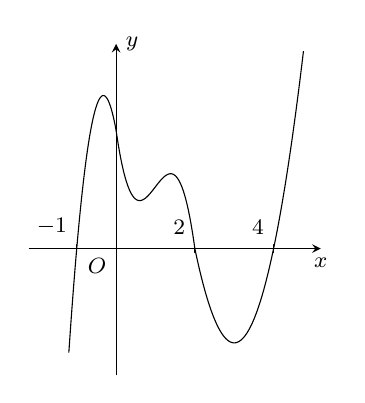
\begin{tikzpicture}[scale=.5, font=\footnotesize, line join=round, line cap=round, >=stealth]
            \def\xmin{-2}\def\xmax{5}\def\ymin{-3}\def\ymax{5}
            \draw[->] (\xmin-0.2,0)--(\xmax+0.2,0) node[below] {\footnotesize $x$};
            \draw[->] (0,\ymin-0.2)--(0,\ymax+0.2) node[right] {\footnotesize $y$};
            \draw (0,0) node [below left] {\footnotesize $O$};
            \foreach \x in {-1,2,4}\draw (\x,-0.1)--(\x,0.1) node [above left] {\footnotesize $\x$};
            \foreach \y in {}\draw (-0.1,\y)--(0.1,\y) node [right] {\footnotesize $\y$};
            \clip (\xmin,\ymin) rectangle (\xmax,\ymax);
            \draw[smooth,samples=200,domain=-1.2:0] plot(\x,{0-8.48*(\x)^(2.0)-5.48*(\x)+3.0});
            \draw[smooth,samples=200,domain=0:2]
            plot(\x,{0-2.7989489689153735*(\x)^(3.0)+8.326740175055514*(\x)^(2.0)-6.957684474449535*(\x)+3.0});
            \draw[smooth,samples=200,domain=2:5]
            plot(\x,{2.395330112721417*(\x)^(2.0)-14.371980676328501*(\x)+19.162640901771336});
    \end{tikzpicture}}
    \loigiai{
        * Điều kiện: $\heva{&f(|x|) \ne 0\\&x \le 3.}$\\
        Nhìn hình vẽ ta thấy
        $f(|x|)=0\Leftrightarrow \hoac{&|x|=-1\\&|x|=2\\&|x|=4}\Leftrightarrow \hoac{&x=\pm 2&(\text{nghiệm đơn})\\&x=- 4&(\text{nghiệm đơn})\\&x=4&(\text{không thỏa mãn}).}$\\
        Vậy $y =\dfrac{(x+2)\sqrt{3-x}}{a(x-2)(x+2)(x+4)(x-4)}$ \\
        Đồ thị hàm số có 2 đường tiệm cận đứng.}
\end{ex}
\begin{ex}
    \immini{ %Câu 94.
        Đường cong ở hình bên là đồ thị của hàm số $y = ax^3 +bx^2 +cx+d$. Đồ thị hàm số $y =\dfrac{(2x+1)\sqrt{1-x}}{f(|x|)}$ có tất cả bao nhiều tiệm cận đứng?
        \choice
        { 1}
        {3}
        {4}
        {\True 2}}{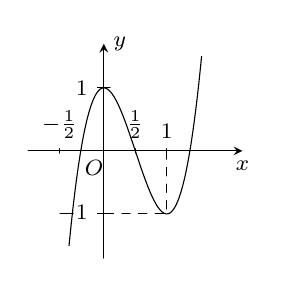
\begin{tikzpicture}[scale=.8, font=\footnotesize, line join=round, line cap=round, >=stealth]
            \def\xmin{-1}\def\xmax{2}\def\ymin{-1.5}\def\ymax{1.5}
            \draw[->] (\xmin-0.2,0)--(\xmax+0.2,0) node[below] {\footnotesize $x$};
            \draw[->] (0,\ymin-0.2)--(0,\ymax+0.2) node[right] {\footnotesize $y$};
            \draw (0.15,0) node [below left] {\footnotesize $O$};
            \foreach \x in {}\draw (\x,0.1)--(\x,-0.1) node [below] {\footnotesize $\x$};
            \foreach \y in {-1,1}\draw (0.1,\y)--(-0.1,\y) node [left] {\footnotesize $\y$};
            \clip (\xmin,\ymin) rectangle (\xmax,\ymax);
            \draw[smooth,samples=200,domain=\xmin:\xmax] plot (\x,{4*((\x)^3)+-6*((\x)^2)+0*(\x)+1});
            \draw[dashed] (0.5,0)--(0.5,0.0)--(0,0.0);
            \draw (0.5,-1pt)--(0.5,1pt) node [above] {\footnotesize $\frac{1}{2}$};
            \draw (-0.7,-1pt)--(-0.7,1pt) node [above] {\footnotesize $-\frac{1}{2}$};
            \draw (1,-1pt)--(1,1pt) node [above] {\footnotesize $1$};
            \draw[dashed] (0.0,0)--(0.0,1.0)--(0,1.0);
            \draw[dashed] (1.0,0)--(1.0,-1.0)--(0,-1.0);
    \end{tikzpicture}}
    \loigiai{
        * Điều kiện: $\heva{&f(|x|) \ne 0\\&x \le 1.}$\\
        Nhìn hình vẽ ta thấy
        $f(|x|)=0\Leftrightarrow \hoac{&|x|=-\dfrac{1}{2}\\&|x|=\dfrac{1}{2}\\&|x|=x_1>1}\Leftrightarrow \hoac{&x=\pm \dfrac{1}{2}&(\text{hai nghiệm đơn})\\&x=- x_1&(\text{nghiệm đơn})\\&x=x_1&(\text{không thỏa mãn}).}$\\
        Vậy $y =\dfrac{(2x+1)\sqrt{1-x}}{f(|x|)}=\dfrac{(2x+1)\sqrt{1-x}}{a\left(x-\dfrac{1}{2}\right)\left(x+\dfrac{1}{2}\right)(x+x_1)(x-x_1)}$ \\
        Đồ thị hàm số có 2 đường tiệm cận đứng.}
\end{ex}
\begin{ex}
    \immini{ %Câu 96.
        Cho đồ thị hàm số $y =f(x)$ và trục hoành có đúng 2 điểm chung như hình bên. Đồ thị hàm số $y =\dfrac{(x-1)\sqrt{3-x}}{f(x^2)}$ có tất cả bao nhiêu tiệm cận đứng?
        \choice
        {1}
        {3}
        {4}
        {\True 2}}{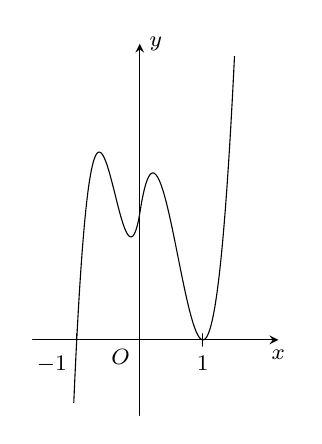
\begin{tikzpicture}[scale=.8, font=\footnotesize, line join=round, line cap=round, >=stealth]
            \def\xmin{-1.5}\def\xmax{2}\def\ymin{-1}\def\ymax{4.5}
            \draw[->] (\xmin-0.2,0)--(\xmax+0.2,0) node[below] {\footnotesize $x$};
            \draw[->] (0,\ymin-0.2)--(0,\ymax+0.2) node[right] {\footnotesize $y$};
            \draw (0,0) node [below left] {\footnotesize $O$};
            \foreach \x in {1}\draw (\x,0.1)--(\x,-0.1) node [below] {\footnotesize $\x$};
            \foreach \x in {-1}\draw (\x,0.1)--(\x,-0.1) node [below left] {\footnotesize $\x$};
            \clip (\xmin,\ymin) rectangle (\xmax,\ymax);
            \draw[smooth,samples=200,domain=-1.1:0] plot(\x,{21.044670464836045*(\x)^(3.0)+24.701786337609526*(\x)^(2.0)+5.65711587277348*(\x)+2.0});
            \draw[smooth,samples=200,domain=0:\xmax] plot(\x,{10.591704641658401*(\x)^(3.0)-19.26315454354621*(\x)^(2.0)+6.6714499018878115*(\x)+2.0});
    \end{tikzpicture}}
    \loigiai{
        * Điều kiện: $\heva{&f(x^2) \ne 0\\&x \le 3.}$\\
        Nhìn hình vẽ ta thấy
        $f(x^2)=0\Leftrightarrow \hoac{&x^2=-1\\&x^2=1}\Leftrightarrow x=\pm 1\,(\text{nghiệm kép}).$\\
        Vậy $y=\dfrac{(x-1)\sqrt{3-x}}{f(x^2)}=\dfrac{(x-1)\sqrt{3-x}}{(x-1)^2(x+1)^2}$ \\
        Đồ thị hàm số có 2 đường tiệm cận đứng.}
\end{ex}
\begin{ex}%[2D1G4-3]%Câu 52
    Cho hàm số $y=ax^3+bx^2+cx+d$ có đồ thị như hình vẽ. Đồ thị của hàm số $g(x)=\dfrac{x^2-x}{f^2(x)-2f(x)}$ có bao nhiêu đường tiệm cận đứng?
    \choice
    {$2$}
    {$3$}
    {\True $4$}
    {$5$}
    \begin{center}
        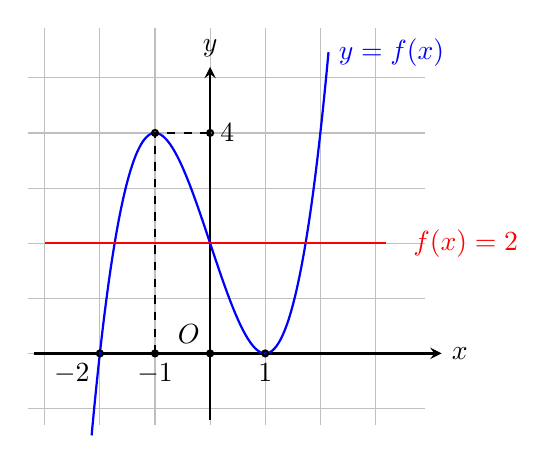
\begin{tikzpicture}[thick,>=stealth,x=1cm,y=1cm,scale=.7]
            \draw[thin,color=gray!50] (-3.3,-1.3) grid (3.9,5.9);
            \draw[->] (-3.2,0) -- (4.2,0) node[right] {$x$};
            \draw[->] (0,-1.2) -- (0,5.2) node[above] {$y$};
            \draw[color=blue, domain=-2.15:2.15,samples=300] plot (\x,{(\x)^3-3*(\x)+2}) node[right] {$y=f(x)$};
            \draw (-2,0) circle (1.5pt) node[below left]{$-2$};
            \draw (-1,0) circle (1.5pt) node[below]{$-1$};
            \draw (0,0) circle (1.5pt) node[above left]{$O$};
            \draw (1,0) circle (1.5pt) node[below]{$1$};
            \draw (0,4) circle (1.5pt) node[right]{$4$};
            \draw (-1,4) circle (1.5pt);
            \draw[dashed] (-1,0)--(-1,4)--(0,4);
            \draw[red] (-3,2)--(3.2,2);
            \draw[red] (3.5,2) node[right]{$f(x)=2$};
        \end{tikzpicture}
    \end{center}
    \loigiai{
        Xét phương trình $f^2(x)-2f(x)=0 \Leftrightarrow \hoac{&f(x)=0\\&f(x)=2}\Leftrightarrow \hoac{&x=1 \, (\textrm{nghiệm kép trùng nghiệm đơn ở tử số})\\&x=-2\, (\textrm{nghiệm đơn khác nghiệm của tử})\\&x=a\in(-2; -1)\\&x=0\, (\textrm{nghiệm đơn trùng nghiệm ở tử})\\&x=b\in(1; 2)}$\\
        \textbf{Kết luận:} Đồ thị hàm số có $4$ đường tiệm cận đứng.
    }
\end{ex}
\begin{ex}%[Thi thử L3, Lương Thế Vinh, Hà Nội, 2018]%[Phạm Toàn, Dự án (12EX-10)]%[2D1G4-3]%
    \immini{Cho hàm số $y=f(x)$ có đạo hàm liên tục trên $\mathbb{R}$. Đồ thị hàm $f(x)$ như hình vẽ. Số đường tiệm cận đứng của đồ thị hàm số $y=\dfrac{x^2-1}{f^2(x)-4f(x)}$ bằng
        \choice
        {$3$}
        {$1$}
        {$2$}
        {\True $4$}
    }{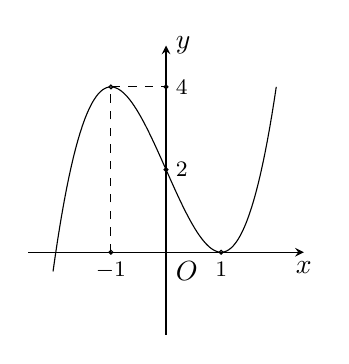
\begin{tikzpicture}[>=stealth,x=1cm,y=0.75cm,scale=0.7]
            \draw[->] (-2.5,0)--(0,0)%
            node[below right]{$O$}--(2.5,0) node[below]{$x$};
            \draw[->] (0,-2) --(0,5) node[right]{$y$};
            \foreach \x in {-1,1}{
                \draw (\x,0) node[below]{\footnotesize $\x$} circle (1pt);%Ox
            }
            \foreach \y in {2,4}{
                \draw (0,\y) node[right]{\footnotesize $\y$} circle (1pt);%Oy
            }
            \draw[samples=100,domain=-2.05:2] plot (\x,{(\x -1)^2*(\x+2)});
            \draw [dashed] (-1,0)--(-1,4)--(0,4);
            \draw(-1,4) circle (1pt);
    \end{tikzpicture}}
    \loigiai{Xét $f^2(x)-4f(x)=0\Leftrightarrow \hoac{& f(x)=0\\ &f(x)=4.}$\\
        Xét $f(x)=0$ có hai nghiệm, nghiệm $x_1\ne \pm 1$ và nghiệm $x_2=1$ là nghiệm bội (do đồ thị tiếp xúc với trục hoành tại $x=1$. Trường hợp này có $2$ tiệm cận đứng.\\
        Xét $f(x)=4$ có hai nghiệm, nghiệm $x_3\ne \pm 1$ và nghiệm $x_4=-1$ là nghiệm bội (do đồ thị tiếp xúc với đường thẳng $y=4$ tại $x=-1$. Trường hợp này có $2$ tiệm cận đứng.\\
        Vậy đồ thị có $4$ tiệm cận đứng.}
\end{ex}
\begin{ex}%[Thi thử, Trường THPT Lý Thái Tổ - Bắc Ninh, 2019]%[Duong Xuan Loi, 12EX3]%[2D1G4-3]%
    \immini{
        Cho hàm số $f(x)$ có đồ thị như hình bên. Số đường tiệm cận đứng của đồ thị hàm số
        $y=\dfrac{(x^2-4)(x^2+2x)}{[f(x)]^2+2f(x)-3}$ là
        \choice
        {\True $4$}
        {$5$}
        {$3$}
        {$2$}
    }{
        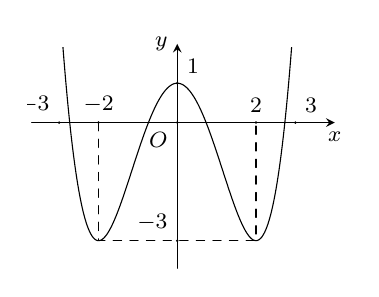
\begin{tikzpicture}[scale=0.5, font=\footnotesize, line join=round, line cap=round, >=stealth]
            \def\a{1} \def\b{-8} \def\c{1} % Hệ số
            \def\xt{-3.7} \def\xp{4} \def\yt{2} \def\yd{-3.7} % x_trái, x_phải, y_trên, y_dưới (giới hạn)
            \draw[->] (\xt,0)--(\xp,0) node [below]{$x$};
            \draw[->] (0,\yd)--(0,\yt) node [left]{$y$};
            \node at (0,0) [below left]{$O$};
            \clip (\xt-0.1,\yd+0.1) rectangle (\xp-0.1,\yt-0.1);
            \draw[smooth,samples=300] plot(\x,{1/4*(\a*(\x)^4+\b*(\x)^2)+\c});
            \draw[dashed] (-2,0)node[above]{$-2$}--(-2,-3)--(2,-3)--(2,0)node[above]{$2$};
            \node at (0,-3)[above left]{$-3$};
            \node at (-3,0)[above left]{$-3$};
            \node at (0,1)[above right]{$1$};
            \node at (3,0)[above right]{$3$};
            \fill (0,0) circle (1pt) (0,-3) circle (1pt) (2,0) circle (1pt) (-2,0) circle (1pt) (-3,0) circle (1pt) (0,1) circle (1pt) (3,0) circle (1pt);
        \end{tikzpicture}
    }
    \loigiai{
        Ta có $y=\dfrac{(x^2-4)(x^2+2x)}{[f(x)]^2+2f(x)-3}$ có các nghiệm ở tử là $x=0$ (bội $1$), $x=2$ (bội $1$), $x=-2$ (bội $2$).\\
        Mặt khác, từ đồ thị $f(x)$ ta thấy hàm số $y=\dfrac{(x^2-4)(x^2+2x)}{[f(x)]^2+2f(x)-3}$ có các nghiệm ở mẫu là
        $f^2(x)+2f(x)-3=0\Leftrightarrow \hoac{& f(x)=1 \\ & f(x)=-3}
        \Leftrightarrow \hoac{& x=0,x=x_1,x=x_2 \\ & x=-2,x=2.}$\\
        Trong đó nghiệm $x=0$, $x=-2$, $x=2$ đều có bội $2$ và $x_1$, $x_2$ khác các nghiệm của tử.\\
        So sánh bội nghiệm ở mẫu và bội nghiệm ở tử thì thấy đồ thị có các tiệm cận đứng là $x=0$, $x=2$; $x=x_1$; $x=x_2$.
    }
\end{ex}
\begin{ex}%[Thi thử, THPT Sơn Tây, Hà Nội, 2019]%[Huỳnh Xuân Tín, 12EX3]%[2D1G4-3]%
    \immini{Cho hàm số $ f(x)=(x+3)(x+1)^2(x-1)(x-3)$ có đồ thị như hình vẽ. Đồ thị hàm số $ g(x)=\dfrac{\sqrt{x-1}}{f^2(x)-9f(x)}$ có bao nhiêu tiệm cận đứng và tiệm cận ngang?
        \choice
        {$3$}
        {\True$ 4$}
        {$ 9$}
        { $8$}
    }{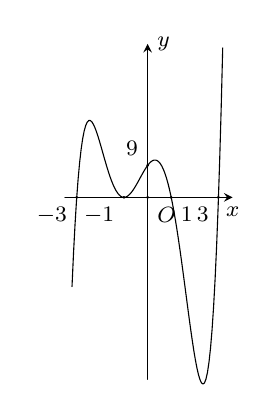
\begin{tikzpicture}[scale=0.3, font=\footnotesize, line join=round, line cap=round, >=stealth]
            %\draw[dashed, line width=0.1pt, gray] (-3.2,-5.5) grid (5.2,4.5);
            \draw[->] (-3.5,0)--(0,0) node[below right]{$O$}--(3.6,0) node[below]{$x$};
            \draw[fill=black] (0,0) circle (1pt);
            \draw[->] (0,-7.7) --(0,6.5) node[right]{$y$};
            \foreach \x in {-3,-1,3}{
                \draw[fill=black] (\x,0) node[below left]{$\x$} circle (1pt);}
            \draw[fill=black] (1,0) node[below right]{$1$} circle (1pt);
            \draw[fill=black] (0,1.35) node[above left]{$9$} circle (1pt);
            \draw [black, domain=-3.2:3.18, samples=100] %
            plot(\x,{0.15*(\x+3)*(\x+1)^2*(\x-1)*(\x-3)});
    \end{tikzpicture}}
    \loigiai{Điều kiện xác định của hàm số $g(x)$ là $\heva{&x\ge1\\ &f^2(x)-9f(x)\not=0.}$\\
        Từ $f^2(x)-9f(x)=0\Leftrightarrow \hoac{&f(x)=0\\&f(x)=9.}$\\
        Với $f(x)=0$ có nghiệm là $x=\pm 1, x=\pm 3$.\\
        Dựa vào đồ thị ta thấy nghiệm của phương trình $f(x)=9$ là hoành độ giao điểm của đường thẳng $y=9$ với đồ thị hàm số $y=f(x)$ nên có nghiệm là $-3<x_3<x_2<-1<0<x_1<1<3<x_0$.\\
        Do đó tập xác định của hàm số $y=g(x)$ là $\mathscr{D}=\left[1;+\infty \right)\setminus\left\lbrace1;3;x_0 \right\rbrace $.\\
        Khi đó ta có \begin{itemize}
            \item $\lim\limits_{x\rightarrow1^+ } g(x)=\lim\limits_{x\rightarrow1^+ }\dfrac{\sqrt{x-1}}{f(x)\left(f(x)-9 \right)}=+\infty$ (vì $x$ tiến gần bên phải $1$ thì $f(x)<0, f(x)-9<0$), suy ra đường thẳng $x=1$ là tiệm cận đứng.
            \item $\lim\limits_{x\rightarrow3^+ } g(x)=\lim\limits_{x\rightarrow3^+ }\dfrac{\sqrt{x-1}}{f(x)\left(f(x)-9 \right)}=-\infty$ (vì $x$ tiến gần bên phải $3$ thì $f(x)>0, f(x)-9<0$), suy ra đường thẳng $x=3$ là tiệm cận đứng.
            \item $\lim\limits_{x\rightarrow x_0^+} g(x)=\lim\limits_{x\rightarrow x_0^+ }\dfrac{\sqrt{x-1}}{f(x)\left(f(x)-9 \right)}=+\infty$ (vì $x$ tiến gần bên phải $x_0$ thì $f(x)>0, f(x)-9>0$), suy ra đường thẳng $x=x_0$ là tiệm cận đứng.
        \end{itemize}
        Và $\lim\limits_{x\rightarrow +\infty} g(x)=\lim\limits_{x\rightarrow +\infty }\dfrac{\sqrt{x-1}}{f(x)\left(f(x)-9 \right)}=0$ (vì bậc ở mẫu của $y=g(x)$ là $10$ và bậc tử của nó là $\dfrac{1}{2}$). Do vậy đồ thị hàm số $y=g(x)$ có một tiệm cận ngang là đường thẳng $y=0$.\\
        Vậy đồ thị hàm số $y=g(x)$ có bốn tiệm cận ngang và đứng. }
\end{ex}
\begin{ex}%[Thi thử, Chuyên Quang Trung-Bình Phước, 2021,lần 1]%[Trần Hòa, 12EX6]%[2D1G4-3]%
    \immini{Cho hàm số $y=f(x)=ax^3+bx^2+cx+d$, có đồ thị như hình vẽ. Số đường tiệm cận đứng của đồ thị hàm số $y=\dfrac{x^2+x-2}{f^2(x)-f(x)}$ là
        \choice
        {$3$}
        {$2$}
        {\True $4$}
        {$5$}}
    {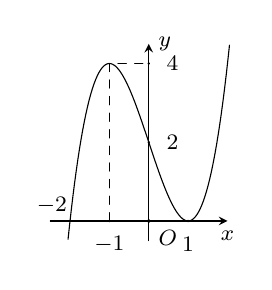
\begin{tikzpicture}[scale=.5, font=\footnotesize, line join=round, line cap=round, >=stealth]
            \draw[->] (-2.5,0)--(0,0) node[below right]{$O$}--(2,0) node[below]{$x$};
            \draw[->] (0,-.5) --(0,4.5) node[right]{$y$};
            \draw [domain=-2.05:2.05, samples=100] %
            plot (\x, {(\x+2)*(\x-1)^2});
            \draw[fill] (0,0) circle (1pt);
            \foreach \x/\g in {-2/140,-1/-90,1/-90}
            \draw[fill] (\x,0) circle(.5pt)node [shift={(\g:.3)}] {$\x$};
            \foreach \y/\g in {2/0,4/0}
            \draw[fill] (0,\y) circle(.5pt)node [shift={(\g:.3)}] {$\y$};
            \draw[dashed] (-1,0)--(-1,4)--(0,4);
    \end{tikzpicture}}
    \loigiai{
        \begin{itemize}
            \item $x^2+x-2=(x-1)(x+2)$.\\
            \item Dựa vào đồ thị hàm số $y=f(x)$ ta có $f^2(x)-f(x)=0\Leftrightarrow\hoac{&f(x)=0\\&f(x)=1.}$\\
            $f(x)=0\Leftrightarrow x=-2$, $x=1$ (nghiệm kép).\\
            $f(x)=1\Leftrightarrow\hoac{&x=x_1,(x_1\in (-2;-1))\\&x=x_2,(x_2\in (0;1))\\&x=x_3,(x_3>1). }$
            \item Do đó $y=\dfrac{(x-1)(x+2)}{a^2(x+2)(x-1)^2(x-x_1)(x-x_2)(x-x_3)}$.
        \end{itemize}
        Suy ra đồ thị có các đườn tiệm cận đứng $x=1$, $x=x_1$, $x=x_2$, $x=x_3$.
    }
\end{ex}
\begin{ex}%[Đề thi hết học kì 2, Bình Minh, Ninh Bình 2018]%[Nguyễn Tuấn Anh, dự án EX9]%[2D1G4-3]%
    \immini{Cho hàm số bậc ba $f(x)=ax^3+bx^2+cx+d$ có đồ thị như hình vẽ bên dưới. Hỏi đồ thị hàm số $g(x)=\dfrac{(x^2-3x+2)\sqrt{x-1}}{x[f^2(x)-f(x)]}$ có bao nhiêu tiệm cận đứng?
        \choice
        {$5$}
        {$6$}
        {\True $3$}
        {$4$}
    }{
        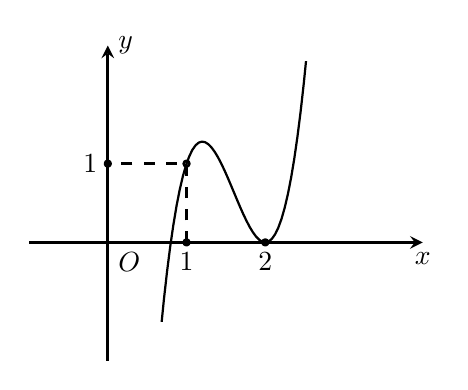
\begin{tikzpicture}[line width=1.0pt,line join=round,>=stealth,x=1cm,y=1cm,scale=1.0]
            \draw[->,line width = 1pt] (-1,0)--(0,0) node[below right]{$O$}--(4,0) node[below]{$x$};
            \draw[->,line width = 1pt] (0,-1.5) --(0,2.5) node[right]{$y$};
            \foreach \x in {1,2}{
                \draw (\x,0) node[below]{$\x$} circle (1pt);
            }
            \foreach \y in {1}{
                \draw (0,\y) node[left]{$\y$} circle (1pt);
            }
            \clip(-0.8,-1) rectangle (3.8,2.3);
            \draw [line width=1.0pt, thick, domain=-0.5:3.5, samples=100]%,domain=-1.5:3] %
            plot (\x, {(5*(\x)-4)*((\x)-2)^2});
            \draw [dash pattern=on 4pt off 4pt] (1.,0.)-- (1.,1.)-- (0.,1.);
            \draw (1,1) circle (1pt);
        \end{tikzpicture}
    }
    \loigiai{
        Điều kiện $\heva{&x\geq 1\\ &x\ne 0\\ &f^2(x)-f(x)\ne 0}\Leftrightarrow \heva{&x\geq 1\\ &f(x)\ne 0\\ & f(x)\ne 1.}$\\
        Dựa vào đồ thị hàm số $y=f(x)$, ta thấy $f(x)=0$ có hai nghiệm, một nghiệm $x_1<1$ và một nghiệm kép bằng $2$. Do đó ta biểu diễn được $f(x)$ dưới dạng
        $$ f(x)=a(x-x_1)(x-2)^2. $$
        Dựa vào đồ thị hàm số $y=f(x)$, ta thấy phương trình $f(x)=1$ có ba nghiệm $1,x_2, x_3$, với $1<x_2<2<x_3$. Do đó ta biểu diễn được $f(x)-1$ dưới dạng
        $$ f(x)-1=a(x-1)(x-x_2)(x-x_3). $$
        Lúc này điều kiện được viết lại như sau $\heva{&x>1\\ &x\ne x_2, x\ne 2, x\ne x_3.}$\\
        Với điều kiện đó thì $g(x)$ được viết lại là
        $$ g(x)=\dfrac{\sqrt{x-1}}{a^2x(x-x_1)(x-x_2)(x-2)(x-x_3)}. $$
        Ta có
        \begin{align*}
            &\lim\limits_{x\to 1^+}g(x)=\lim\limits_{x\to 1^+}\dfrac{\sqrt{x-1}}{a^2x(x-x_1)(x-x_2)(x-2)(x-x_3)}=0,\\
            & (x=1\mbox{ \textbf{không} là tiệm cận đứng}) \\
            &\lim\limits_{x\to x_2^+}g(x)=\lim\limits_{x\to x_2^+}\dfrac{\sqrt{x-1}}{a^2x(x-x_1)(x-x_2)(x-2)(x-x_3)}=+\infty,\\
            & (x=x_2\mbox{ là tiệm cận đứng}) \\
            &\lim\limits_{x\to 2^+}g(x)=\lim\limits_{x\to 2^+}\dfrac{\sqrt{x-1}}{a^2x(x-x_1)(x-x_2)(x-2)(x-x_3)}=-\infty,\\
            & (x=2\mbox{ là tiệm cận đứng}) \\
            &\lim\limits_{x\to x_3^+}g(x)=\lim\limits_{x\to x_3^+}\dfrac{\sqrt{x-1}}{a^2x(x-x_1)(x-x_2)(x-2)(x-x_3)}=+\infty,\\
            & (x=x_3\mbox{ là tiệm cận đứng}) \\
        \end{align*}
        Vậy đồ thị hàm số $g(x)$ có tất cả $3$ tiệm cận đứng.
    }
\end{ex}
\begin{ex}%[VDC5-Đỗ Đường Hiếu]%[2D1G4-3]%
    \immini{Cho hàm số $f(x)=(x+3)(x+1)^2(x-1)(x-3)$ có đồ thị như hình vẽ. Đồ thị hàm số $g(x)=\dfrac{\sqrt{x-1}}{f^2(x)-9f(x)}$ có bao nhiêu tiệm cận đứng và tiệm cận ngang?
        \choice
        {$3$}
        {\True $4$}
        {$9$}
        {$8$}}
    {\begin{tikzpicture}[xscale=0.8,yscale=0.05, line join=round, line cap=round,font=\footnotesize,>=stealth]
            \draw[->] (-4,0)--(4,0) node[below]{$x$};
            \draw[->] (0,-56)--(0,30) node[left]{$y$};
            \coordinate[label=below left:$O$] (O) at (0,0);
            \draw (-1,0) node[below] { $-1$}(1,0) node[below] { $1$};
            \draw (-3,0) node[below left] { $-3$};
            \draw (3,0) node[below right] { $3$};
            \clip (-3.3,-60) rectangle (3.5,26);
            \draw[smooth,samples=300,domain=-3.5:3.5] plot(\x,{(\x+3)*(\x+1)^2*(\x-1)*(\x-3)});
            \foreach \x in {-3,-1,1,3}
            \draw[shift={(\x,0)},color=black] (0pt,20pt) -- (0pt,-20pt);
            \draw[shift={(0,9)},color=black] (2pt,0pt) -- (-2pt,0pt) node[left] {$9$};
        \end{tikzpicture}
    }
    \loigiai{%GV tổng quát hóa bài toán:
        Cho hàm số đa thức $y=f(x)$ có đồ thị $(C)$. Tìm số đường tiệm cận của đồ thị hàm số $g(x)=\dfrac{\sqrt{ax+b}}{P\left(f(x) \right) }$, trong đó $P\left(f(x) \right)$ là một đa thức của $f(x)$.
        Nếu $a>0$ thì $\lim\limits_{x\to +\infty}g(x)=0$.\\
        Nếu $a<0$ thì $\lim\limits_{x\to -\infty}g(x)=0$.\\
        Do đó đồ thị hàm số $y=g(x)$ luôn có duy nhất một đường tiệm cận ngang là $y=0$.\\
        Gọi $x=x_0$ là một nghiệm của phương trình $P\left(f(x) \right) =0$ thỏa mãn điều kiện $ax+b\ge 0$. Rõ ràng khi đó $\lim\limits_{x\to x_0^+}g(x)=+\infty$ hoặc $\lim\limits_{x\to x_0^+}g(x)=-\infty$.\\
        Bởi vậy, số đường tiệm cận đứng của đồ thị hàm số $y=g(x)$ chính là số nghiệm của phương trình $P\left(f(x) \right) =0$ thỏa mãn điều kiện $ax+b\ge 0$.
        \immini{Ta có $f^2(x)-9f(x)=0\Leftrightarrow \hoac{&f(x)=0\\&f(x)=9.}$\\
            \begin{itemize}
                \item $f(x)=0$ có các nghiệm thuộc $\left[1;+\infty\right)$ là $x=1$ và $x=3$.
                \item Đường thẳng $y=9$ cắt đồ thị hàm số $y=f(x)$ tại duy nhất một điểm có hoành độ thuộc $\left[1;+\infty\right)$ là $x=a>3$.
            \end{itemize}
        }
        {\begin{tikzpicture}[xscale=0.8,yscale=0.05, line join=round, line cap=round,font=\footnotesize,>=stealth]
                \draw[->] (-4,0)--(4,0) node[below]{$x$};
                \draw[->] (0,-56)--(0,30) node[left]{$y$};
                \coordinate[label=below left:$O$] (O) at (0,0);
                \draw (-4,9)--(4,9);
                \draw (-1,0) node[below] { $-1$}(1,0) node[below] { $1$};
                \draw (-3,0) node[below left] { $-3$};
                \draw (3,0) node[below right] { $3$};
                \clip (-3.3,-60) rectangle (3.5,26);
                \draw[smooth,samples=300,domain=-3.5:3.5] plot(\x,{(\x+3)*(\x+1)^2*(\x-1)*(\x-3)});
                \foreach \x in {-3,-1,1,3}
                \draw[shift={(\x,0)},color=black] (0pt,20pt) -- (0pt,-20pt);
                \draw[shift={(0,9)},color=black] (2pt,0pt) -- (-2pt,0pt) node[above left] {$9$};
        \end{tikzpicture}}
        \noindent
        Bởi vậy, hàm số $g(x)=\dfrac{\sqrt{x-1}}{f^2(x)-9f(x)}$ có tập xác định là $\mathscr D=\left[1;3\right) \cup \left(3;a\right) \cup\left( a;+\infty\right)$.\\
        Khi đó ta có
        \begin{itemize}
            \item $\lim\limits_{x\to+\infty}g(x)=0$ nên đồ thị hàm số $y=g(x)$ có một đường tiệm cận ngang là đường thẳng $y=0$.
            \item $\lim\limits_{x\to 1^+}g(x)=\lim\limits_{x\to 1^+}\dfrac{\sqrt{x-1}}{f(x)\left[f(x)-9\right] }=+\infty$;\\
            $\lim\limits_{x\to 3^+}g(x)=\lim\limits_{x\to 3^+}\dfrac{\sqrt{x-1}}{f(x)\left[f(x)-9\right] }=-\infty$;\\
            $\lim\limits_{x\to a^+}g(x)=\lim\limits_{x\to a^+}\dfrac{\sqrt{x-1}}{f(x)\left[f(x)-9\right] }=+\infty$.\\
            Do đó nên đồ thị hàm số $y=g(x)$ có $3$ đường tiệm cận đứng là các đường thẳng $x=1$, $x=3$ và $x=a$.
        \end{itemize}
        Như vậy, đồ thị hàm số $y=g(x)$ có $4$ đường tiệm cận, trong đó có $1$ đường tiệm cận ngang và $3$ đường tiệm cận đứng.
    }
\end{ex}
\begin{ex}%[VDC5-Đỗ Đường Hiếu]%[2D1G4-3]%
    \immini{Cho hàm số bậc ba $y=f(x)$ có đồ thị như hình vẽ bên. Đồ thị hàm số $g(x)=\dfrac{x\sqrt{x+1}}{f(x)\left[f^2(x)-16 \right] }$ có bao nhiêu tiệm cận đứng?
        \choice
        {\True $4$}
        {$5$}
        {$6$}
        {$7$}}
    {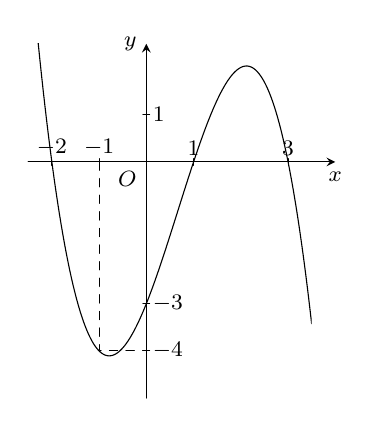
\begin{tikzpicture}[scale=0.6,line join=round, line cap=round,font=\footnotesize,>=stealth]
            \draw[->] (-2.5,0)--(4,0) node[below]{$x$};
            \draw[->] (0,-5)--(0,2.5) node[left]{$y$};
            \coordinate[label=below left:$O$] (O) at (0,0);
            \draw[dashed] (-1,0)--(-1,-4)--(0,-4);
            \clip (-2.3,-5) rectangle (3.5,2.5);
            \draw[smooth,samples=300,domain=-3.5:3.5] plot(\x,{-0.5*(\x+2)*(\x-1)*(\x-3)});
            \foreach \x in {-2,-1,1,3}
            \draw[shift={(\x,0)},color=black] (0pt,2pt) -- (0pt,-2pt) node[above] { $\x$};
            \foreach \y in {-4,-3,1}
            \draw[shift={(0,\y)},color=black] (2pt,0pt) -- (-2pt,0pt) node[right] {$\y$};
        \end{tikzpicture}
    }
    \loigiai{
        Xét phương trình $f(x)\left[f^2(x)-16 \right]=0$ \, $(*)$, với điều kiện $x\in\left[-1;+\infty \right) $.\\
        Ta có $f(x)\left[f^2(x)-16 \right]=0\Leftrightarrow \hoac{&f(x)=0\\&f(x)=4\\&f(x)=-4.}$\\
        \begin{itemize}
            \item Phương trình $f(x)=0$ có hai nghiệm $x\in\left[-1;+\infty \right) $ là $x=1$ và $x=3$.
            \item Phương trình $f(x)=4$ có không có nghiệm $x\in\left[-1;+\infty \right) $.
            \item Phương trình $f(x)=-4$ có hai nghiệm $x\in\left[-1;+\infty \right) $ là $-1<x_1<0$ và $x_2>3$.
        \end{itemize}
        Rõ ràng $\lim\limits_{x\to x_0^+}g(x)=+\infty$ hoặc $\lim\limits_{x\to x_0^+}g(x)=-\infty$, trong đó $x=x_0$ là nghiệm thuộc $\left[-1;+\infty \right) $ của phương trình $(*)$. Do đó đường thẳng $x=x_0$ là tiệm cận đứng của đồ thị hàm số $y=g(x)$.\\
        Từ đó suy ra đồ thị hàm số $g(x)=\dfrac{x\sqrt{x+1}}{f(x)\left[f^2(x)-16 \right] }$ có $4$ tiệm cận đứng.
    }
\end{ex}
\begin{ex}%[VDC5-Đỗ Đường Hiếu]%[2D1G4-3]%
    \immini{Cho $y=f(x)$ là hàm số đa thức có đồ thị như hình vẽ bên. Đặt $g(x)=\dfrac{\sqrt{x-1}}{\left[f(x)\right]^2-2f(x)}$ có bao nhiêu đường tiệm cận đứng?
        \choice
        {$5$}
        {$3$}
        {$4$}
        {\True $2$}}
    {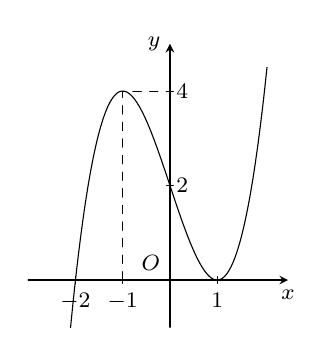
\begin{tikzpicture}[scale=0.6,line join=round, line cap=round,font=\footnotesize,>=stealth]
            \draw[->] (-3,0)--(2.5,0) node[below]{$x$};
            \draw[->] (0,-1)--(0,5) node[left]{$y$};
            \coordinate[label=above left:$O$] (O) at (0,0);
            \draw[dashed] (-1,0)--(-1,4)--(0,4);
            \clip (-2.3,-1) rectangle (2.5,4.5);
            \draw[smooth,samples=300,domain=-3.5:3.5] plot(\x,{(\x)^3-3*(\x)+2});
            \foreach \x in {-2,-1,1}
            \draw[shift={(\x,0)},color=black] (0pt,2pt) -- (0pt,-2pt) node[below] { $\x$};
            \foreach \y in {2,4}
            \draw[shift={(0,\y)},color=black] (2pt,0pt) -- (-2pt,0pt) node[right] {$\y$};
        \end{tikzpicture}
    }
    \loigiai{
        Xét phương trình $\left[f(x)\right]^2-2f(x)=0$ \, $(*)$, với điều kiện $x\in\left[1;+\infty \right) $.\\
        Ta có $\left[f(x)\right]^2-2f(x)=0\Leftrightarrow \hoac{&f(x)=0\\&f(x)=2.}$\\
        \begin{itemize}
            \item Phương trình $f(x)=0$ có một nghiệm $x\in\left[1;+\infty \right) $ là $x=1$.
            \item Phương trình $f(x)=2$ có một nghiệm $x\in\left[1;+\infty \right) $ là $x=x_1>1$.
        \end{itemize}
        Rõ ràng $\lim\limits_{x\to x_0^+}g(x)=+\infty$ hoặc $\lim\limits_{x\to x_0^+}g(x)=-\infty$, trong đó $x=x_0$ là nghiệm thuộc $\left[1;+\infty \right) $ của phương trình $(*)$. Do đó đường thẳng $x=x_0$ là tiệm cận đứng của đồ thị hàm số $y=g(x)$.\\
        Từ đó suy ra đồ thị hàm số $g(x)=\dfrac{\sqrt{x-1}}{\left[f(x)\right]^2-2f(x)}$ có $2$ tiệm cận đứng.
    }
\end{ex}
\begin{ex}%[VDC5-NgocDungHo]%[2D1G4-3]%
    \immini
    {
        Cho hàm số $f(x)$ có đồ thị như hình bên. Số đường tiệm cận đứng của đồ thị hàm số $y=\dfrac{(x^2-4)(x^2+2x)}{[f(x)]^2-4f(x)+3}$ là
        \choice
        {$4$}
        {\True $5$}
        {$3$}
        {$2$}
    }
    {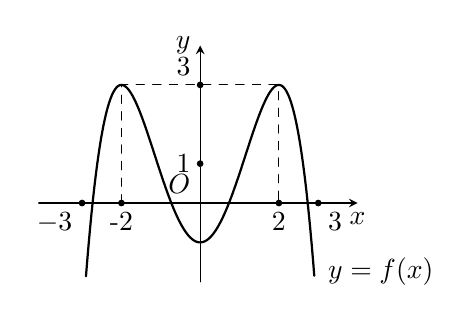
\begin{tikzpicture}[>=stealth,scale=0.5, line join=round, line cap=round]
            \def\f[#1]{-0.25*((#1)^4-8*(#1)^2+4)}
            \draw[->] (-4.1,0)--(4,0) node [below]{$x$};
            \draw[->] (0,-2)--(0,4) node [left]{$y$};
            \node at (0,0) [above left]{$O$};
            % \clip;
            \draw[domain=-2.9:2.9,samples=300,thick] plot (\x,{\f[\x]});
            \foreach \x in {-2,2} \filldraw (\x,0) node[below]{\x} circle (2pt);
            %\foreach \x in {-3,3} \filldraw (\x,0) node[below left]{\x} circle (2pt);
            \filldraw (-3,0) node[below left]{$-3$} circle (2pt);
            \filldraw (3,0) node[below right]{$3$} circle (2pt);
            \filldraw (0,1) node[left]{$1$} circle (2pt);
            \filldraw (0,3) node[above left]{$3$} circle (2pt);
            \draw[dashed](-2,0)--(-2,3)--(2,3)--(2,0);
            \draw (3,-1.75) node[right]{$y=f(x)$};
        \end{tikzpicture}
    }
    \loigiai{
        Xét hàm số $y=g(x)=\dfrac{(x^2-4 )(x^2+2x)}{[f(x)]^2-4f(x)+3}$.
        \immini
        {
            Giải phương trình $(x^2-4)(x^2+2x)=0 $\\
            $\Leftrightarrow \hoac{& x^2-4=0 \\ & x^2+2x=0}\Leftrightarrow \hoac{& x=\pm 2 \\ & x=0.}$\\
            Giải phương trình $[f(x)]^2-4f(x)+3=0$\\
            $ \Leftrightarrow \hoac{& f(x)=1 \\ & f(x)=3} \Leftrightarrow \hoac{& x = \pm 2 \\ & x=a\\&x=b\\&x=c\\&x=d.}$\\ với $-3<a<-2<b<c<2<d<3$.\\
        }
        {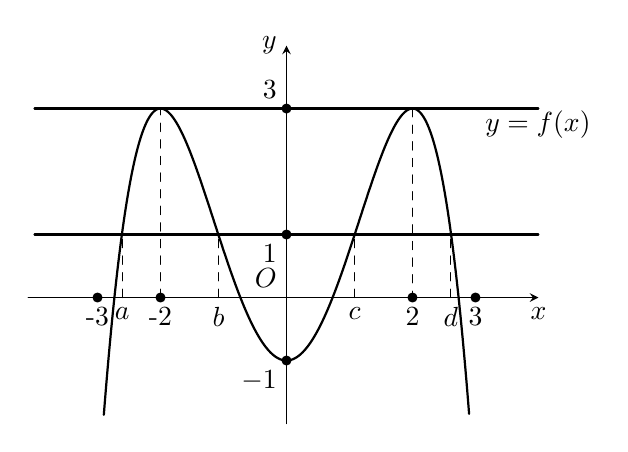
\begin{tikzpicture}[>=stealth,scale=0.8, line join=round, line cap=round]
                \def\f[#1]{-0.25*((#1)^4-8*(#1)^2+4)}
                \def\g[#1]{1}
                \def\h[#1]{3}
                \draw[->] (-4.1,0)--(4,0) node [below]{$x$};
                \draw[->] (0,-2)--(0,4) node [left]{$y$};
                \node at (0,0) [above left]{$O$};
                % \clip;
                \draw[domain=-2.9:2.9,samples=300,thick] plot (\x,{\f[\x]});
                \draw[domain=-4:4,samples=300,thick] plot (\x,{\g[\x]});
                \draw[domain=-4:4,samples=300,thick] plot (\x,{\h[\x]});
                \foreach \x in {-3,-2,2,3} \filldraw (\x,0) node[below]{\x} circle (2pt);
                % \filldraw (-3,0) node[above left]{$-3$} circle (2pt);
                % \filldraw (3,0) node[above ]{$3$} circle (2pt);
                \filldraw (0,1) node[below left]{$1$} circle (2pt);
                \filldraw (0,-1) node[below left]{$-1$} circle (2pt);
                \filldraw (0,3) node[above left]{$3$} circle (2pt);
                \draw[dashed](-2,0)--(-2,3) (2,3)--(2,0) (2.61,0)node[below]{$d$}--(2.61,1) (-2.61,0)node[below]{$a$}--(-2.61,1) (1.08,0)node[below]{$c$}--(1.08,1)(-1.08,0)node[below]{$b$}--(-1.08,1);
                \draw (3,2.75) node[right]{$y=f(x)$};
            \end{tikzpicture}
        }
        Trong điều kiện xác định của hàm số $y=g(x)$ ta có thể viết $$y=g(x)=\dfrac{x(x-2)(x+2)^2}{(x-a)(x-b)(x-c)(x-d) (x-2)^2(x+2)^2}=\dfrac{x}{(x-a)(x-b)(x-c)(x-d)(x-2)}$$
        Vậy số tiệm cận đứng của đồ thị hàm số $y=g(x)$ bằng $5$.
    }
\end{ex}
\Closesolutionfile{ans}